% !TeX root = ../main.tex
\chapter{Introduction}

Text-to-image (T2I) models can produce detailed images from very short
natural-language prompts. Their outputs may be visually coherent and
aesthetically convincing, but visual plausibility does not imply factual
knowledge. A model may generate a plausible castle, animal, or portrait without
knowing which properties distinguish the requested entity from related entities.
It may also add contextual details that are not supported by the entity's
real-world description.

This distinction matters when generated images are used for educational
material, search interfaces, knowledge bases, or other multimodal applications.
In these settings, an image may be interpreted as an assertion about the entity.
An incorrect tower shape, an invented historical attribute, or an unrelated
object can therefore turn a visually attractive image into misleading
information.

This thesis studies factual knowledge in T2I models rather than general visual
quality. It builds on the scalable knowledge-base illustration pipeline
developed by Brinster~\citep{brinster2025}, but changes the objective from
illustrating a large knowledge base to measuring what image-generation models
know about individual entities. The benchmark uses identical zero-context
prompts for all models, preventing the prompt from providing the facts being
measured.

\section{Research Questions}

The thesis addresses three research questions:

\begin{description}[leftmargin=2.8cm,style=nextline]
\item[RQ1:] For how many real-world entities can T2I models correctly predict
their type?
\item[RQ2:] For how many real-world entities do T2I models know descriptive
features that distinguish them from related entities?
\item[RQ3:] Of the facts expressed in generated images for a given entity, how
many are true?
\end{description}

RQ1 measures coarse entity recognition. RQ2 tests whether the image contains a
feature more informative than a generic category label. RQ3 evaluates factuality
at proposition level and accounts for the fact that models may produce different
numbers of visual claims per image.

\section{Contributions}

This thesis introduces a benchmark with curated and randomly sampled real-world
entities, including a popularity-tier split for studying Long-tail behaviour. It
implements a reproducible generation pipeline using one zero-context prompt
across three T2I models and a two-stage visual evaluation pipeline separating
blind type and feature judgments from proposition-based factuality checking. It
also reports model coverage, safety refusals, missing evaluations, proposition
counts, and hallucination rates rather than successful outputs alone.

\section{Thesis Structure}

Chapter~2 reviews T2I models, factuality evaluation, hallucinations, and
knowledge-base illustration. Chapter~3 describes the benchmark, generation
procedure, evaluation protocol, and metrics. Chapter~4 reports the results.
Chapter~5 discusses the findings and limitations. Chapter~6 concludes the thesis
and outlines future work.

\chapter{Related Work}

\section{Text-to-Image Models}

Diffusion models iteratively transform noise into an image. The process is
conditioned on a text representation~\citep{rombach2022}. Commercial systems
and open or hosted models represent different deployment settings, including
centrally operated systems with safety filtering and models with greater control
over generation.

The ability to produce a plausible image should not be confused with knowledge
of the prompt entity. T2I generation is underdetermined: many images can be
compatible with a short prompt, and the model is free to fill in omitted details.
This makes factual evaluation important for historical figures, rare species,
cultural objects, and entities easily confused with related concepts.

\section{Knowledge Bases and Visual Representations}

Knowledge bases represent entities and relations in structured form. A visual
representation can make an entity easier to recognize, but it also introduces a
new surface on which incorrect information can appear. Earlier work demonstrated
that triples can be transformed into image prompts for knowledge-base completion
at scale~\citep{abuahmad2023}. Brinster~\citep{brinster2025} extended this
direction to a large-scale illustration pipeline and investigated image quality,
reuse, scalability, and bias. The current thesis follows that line of research
but uses the generated image as an object of factual evaluation.

\section{Evaluating Visual Factuality}

Pixel-level metrics can measure properties such as sharpness or visual similarity,
but they do not determine whether an image contains the right entity or a false
attribute. CLIP-based similarity is useful for broad image alignment
\citep{hessel2021}, yet a high similarity score can hide an important factual
error. Proposition-based evaluation instead decomposes a description into atomic
claims and verifies each claim against a reference. This thesis adopts that
principle and uses a vision-language judge in a blind description and grounded
verification pipeline.

\section{Hallucinations and Long-Tail Entities}

In this work, a hallucination is an image proposition unsupported by or
contradicted by the reference description. The definition is tied to an explicit
reference rather than to an evaluator's general expectation. The benchmark
therefore reports both the number of propositions generated and the fraction
classified as hallucinations.

\chapter{Methodology}

\section{Benchmark Design}

The benchmark contains 298 entities. The curated subset consists of four domains:
Famous Landmarks and Architecture, Historical Figures, Rare Flora and Fauna, and
Specific Cultural Artifacts and Foods. Each domain contains 25 entities, giving
100 curated entities. The remaining 198 entities form the Random subset, divided
into approximately equal Famous, Medium, and Long-tail popularity tiers.

For curated entities, the benchmark provides an expected type and a distinctive
feature. For Random entities, these fields are intentionally undefined.
Consequently, RQ1 and RQ2 are evaluated only on curated entities, while RQ3 is
evaluated on both curated and Random entities.

Table~\ref{tab:benchmark-composition} summarizes the composition of the
benchmark. The curated categories were chosen to cover architecture, people,
biology, and culturally specific objects. This makes it possible to distinguish
general visual competence from knowledge that is concentrated in a particular
domain. The Random subset provides a broader test of entities that are not
necessarily represented by a canonical visual prototype.

\begin{table}[ht]
\centering
\caption{Composition of the factuality benchmark.}
\label{tab:benchmark-composition}
\begin{tabular}{lrr}
\toprule
Subset or category & Entities & RQ1/RQ2 annotations \\
\midrule
Famous Landmarks and Architecture & 25 & Type and feature \\
Historical Figures & 25 & Type and feature \\
Rare Flora and Fauna & 25 & Type and feature \\
Specific Cultural Artifacts and Foods & 25 & Type and feature \\
Random: Famous tier & 66 & Not defined \\
Random: Medium tier & 66 & Not defined \\
Random: Long-tail tier & 66 & Not defined \\
\midrule
Total & 298 & -- \\
\bottomrule
\end{tabular}
\end{table}

\section{Prompting and Image Generation}

Every entity is presented with the same prompt template:

\begin{quote}
\texttt{An image of [entity].}
\end{quote}

No type, feature, Wikipedia text, or additional visual description is included.
Images were generated with GPT Image 2, FLUX.2-dev, and FLUX.2-klein-4B. The
generation script stores images by model and entity and skips existing files so
interrupted runs can be resumed without duplicating requests.

\section{Visual Evaluation Pipeline}

The evaluation uses two stages. First, the judge model receives the image without
the entity name and produces a description, predicted type, and feature judgment.
The predictions are compared with the curated benchmark annotations for RQ1 and
RQ2. Second, the judge produces atomic propositions describing visible facts.
Each proposition is checked against a Wikipedia lead summary for the entity.

The evaluator records the number of propositions and hallucinations. The main
normalized metric is

\begin{equation}
\mathrm{HallucinationRate}(m) =
\frac{\sum_i H_{i,m}}{\sum_i P_{i,m}},
\end{equation}

where $H_{i,m}$ is the hallucination count for image $i$ generated by model $m$,
and $P_{i,m}$ is the number of propositions generated for that image.

For RQ1, a result is correct if the predicted type matches the benchmark's
expected type. For RQ2, a result is correct if the evaluator determines that the
annotated distinctive feature is visibly present. These metrics are binary and
are reported as the mean of the corresponding indicator variable. For RQ3, the
binary decision is made at proposition level before aggregation. A proposition
that is not supported by the reference or that contradicts it contributes one
hallucination. This approach avoids treating an image with ten correct and one
incorrect claim as equivalent to an image with only one incorrect claim.

\section{Fair Comparison and Missing Evaluations}

Comparing only successful outputs can be misleading when models have unequal
coverage. The main comparison therefore uses the intersection of entity sets
available for all three models. Available-case tables are retained for
transparency, while fair-comparison tables use the 289 common entities. Nine
GPT Image 2 generations were refused by the provider's safety system. These
entries are recorded as missing evaluations and are not counted as either
correct or incorrect model outputs.

\section{Fact-Count Analysis}

The number of propositions is itself informative. A short description has fewer
opportunities to hallucinate, but may also convey less information. The analysis
therefore reports average propositions by model and popularity tier, total
propositions, raw hallucination counts, and normalized rates. Spearman
correlations are used descriptively to examine whether verbosity is associated
with hallucination count or image-level hallucination rate.

\chapter{Results}

\section{Dataset Coverage}

The evaluation file contains 885 successful image evaluations: 289 for GPT Image
2 and 298 for each FLUX model. The nine missing GPT Image 2 evaluations are all
safety refusals. Since the refusals are concentrated in one model, the fair
comparison is based on the 289 entities present for every model.

\section{Type and Feature Recognition}

On the curated subset, the available-case type-match rates are 77.3\% for GPT
Image 2, 80.0\% for FLUX.2-dev, and 73.0\% for FLUX.2-klein-4B. On the common
curated subset, the corresponding rates are 77.3\%, 79.4\%, and 73.2\%.
FLUX.2-dev therefore achieves the strongest coarse type recognition in this
benchmark.

Distinctive feature presence shows a different ranking. GPT Image 2 reaches
62.9\% on the common curated subset, followed by FLUX.2-dev at 46.4\% and
FLUX.2-klein-4B at 28.9\%. Correct type recognition is therefore not sufficient
for recovering entity-specific visual information.

\section{Hallucination Rates}

On the common 289-entity set, the overall hallucination rates are 9.0\% for GPT
Image 2, 9.7\% for FLUX.2-dev, and 17.7\% for FLUX.2-klein-4B. The mean number
of hallucinations per image is 0.70, 0.69, and 1.32, respectively.

The popularity split reveals a more detailed pattern. GPT Image 2 has rates of
3.0\% for Famous entities, 7.3\% for Medium entities, and 23.0\% for Long-tail
entities. For FLUX.2-dev, the rates are 10.9\%, 8.0\%, and 14.6\%; for
FLUX.2-klein-4B, they are 22.8\%, 15.9\%, and 21.1\%.

\section{Number of Generated Facts}

On the fair common set, FLUX.2-dev generates 7.61 propositions per Famous image,
7.30 per Medium image, and 6.95 per Long-tail image. FLUX.2-klein-4B generates
7.75, 7.70, and 7.51 propositions, respectively. GPT Image 2 generates 8.33,
8.25, and 7.69 propositions. Long-tail images therefore tend to contain fewer
described facts, especially for the FLUX models.

The relationship between proposition count and hallucination rate is weak. The
Spearman correlations with image-level hallucination rate are 0.10 for GPT Image
2, 0.06 for FLUX.2-dev, and 0.08 for FLUX.2-klein-4B. Generating fewer facts
does not automatically make an image more factual.

\begin{figure}[ht]
\centering
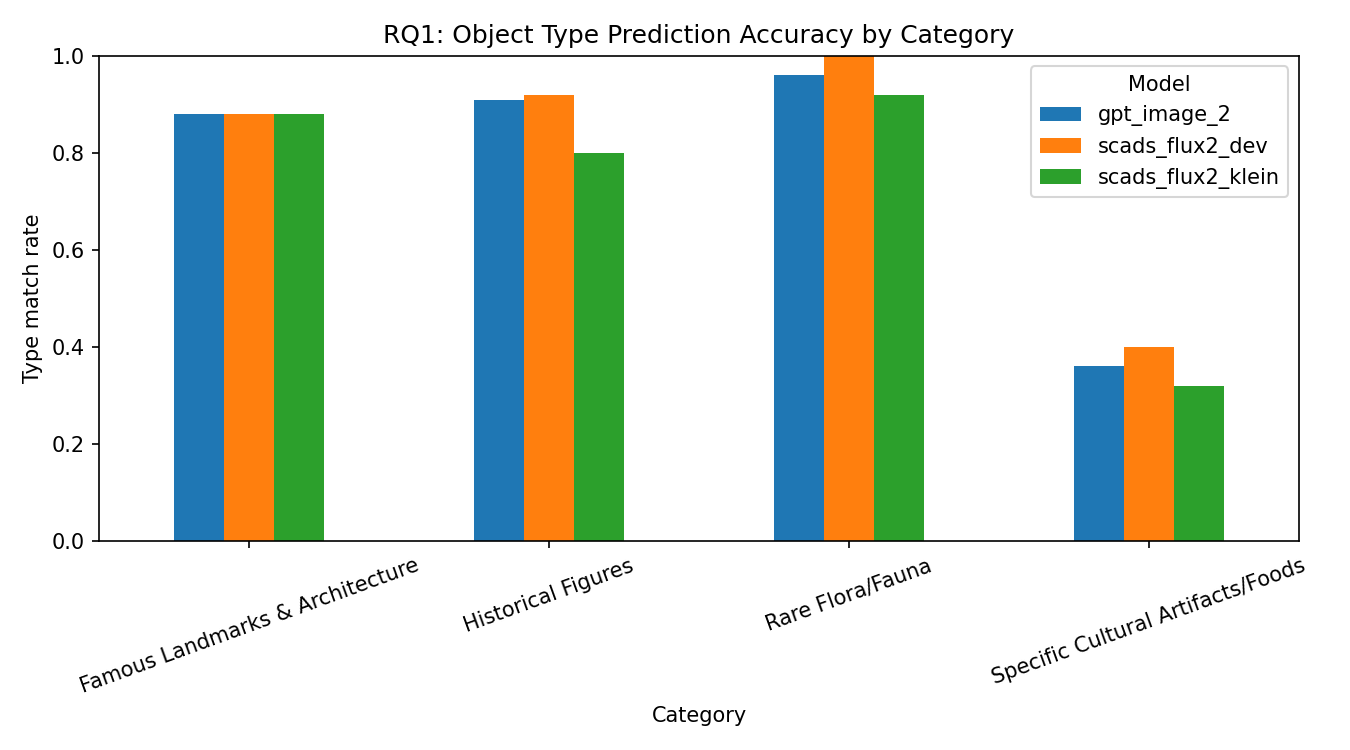
\includegraphics[width=0.82\textwidth]{../Code/analysing/analysis_output/rq1_type_match_by_category.png}
\caption{Type-match rates by curated category and model.}
\label{fig:rq1-category}
\end{figure}

\begin{figure}[ht]
\centering
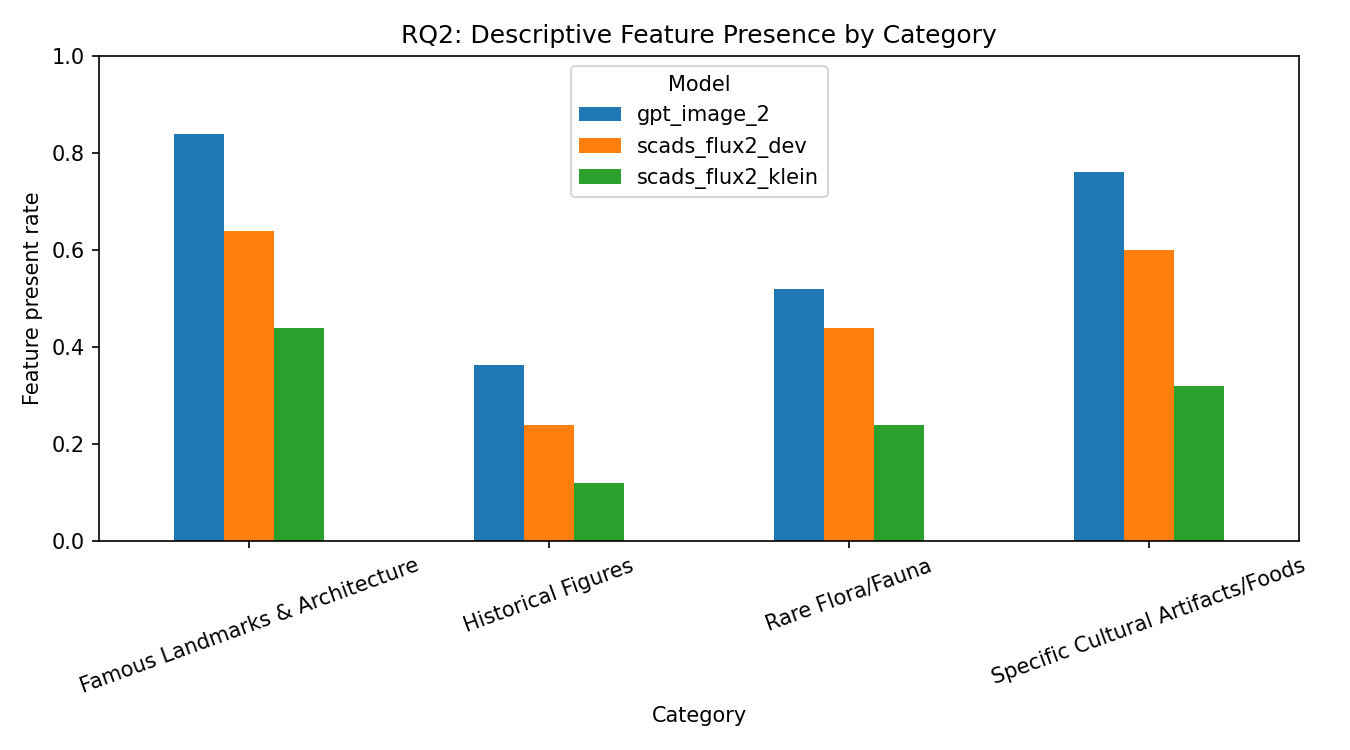
\includegraphics[width=0.82\textwidth]{../Code/analysing/analysis_output/rq2_feature_present_by_category.png}
\caption{Distinctive-feature presence by curated category and model.}
\label{fig:rq2-category}
\end{figure}

Figures~\ref{fig:rq1-category} and~\ref{fig:rq2-category} show why the overall
means should be interpreted together with category-level results. Type
recognition is strongest for flora and fauna, while feature presence varies much
more between domains. In particular, culturally specific artifacts and foods
remain difficult even when the output can sometimes be assigned to the broad
type ``object.''

\begin{table}[ht]
\centering
\caption{Fair comparison on the 289 entities available for every model.}
\label{tab:fair-overall}
\begin{tabular}{lrrrrr}
\toprule
Model & RQ1 & RQ2 & Avg. hallucinations & Avg. facts & Hallucination rate \\
\midrule
GPT Image 2 & 77.3\% & 62.9\% & 0.70 & 7.70 & 9.0\% \\
FLUX.2-dev & 79.4\% & 46.4\% & 0.69 & 7.13 & 9.7\% \\
FLUX.2-klein-4B & 73.2\% & 28.9\% & 1.32 & 7.45 & 17.7\% \\
\bottomrule
\end{tabular}
\end{table}

Table~\ref{tab:fair-overall} is the primary model comparison. It uses the same
entity set for every model and therefore avoids interpreting the nine refused
GPT Image 2 prompts as either successes or failures. The table also makes clear
that no single model dominates every metric: FLUX.2-dev has the highest type
accuracy, GPT Image 2 has the highest feature rate, and GPT Image 2 and
FLUX.2-dev are close in normalized hallucination rate.

\begin{table}[ht]
\centering
\caption{Hallucination rate by popularity tier on the common entity set.}
\label{tab:tier-hallucination}
\begin{tabular}{lrrr}
\toprule
Popularity tier & GPT Image 2 & FLUX.2-dev & FLUX.2-klein-4B \\
\midrule
Famous & 3.0\% & 10.9\% & 22.8\% \\
Medium & 7.3\% & 8.0\% & 15.9\% \\
Long-tail & 23.0\% & 14.6\% & 21.1\% \\
\bottomrule
\end{tabular}
\end{table}

The tier-level comparison in Table~\ref{tab:tier-hallucination} suggests that
popularity affects models differently. GPT Image 2 shows a pronounced increase
for Long-tail entities. FLUX.2-dev has a smaller increase, while FLUX.2-klein-4B
remains comparatively error-prone in all tiers. This is consistent with the
interpretation that models can often produce a generic visual category for a
rare entity while failing to preserve the entity-specific facts that would make
the image informative.

\begin{figure}[ht]
\centering
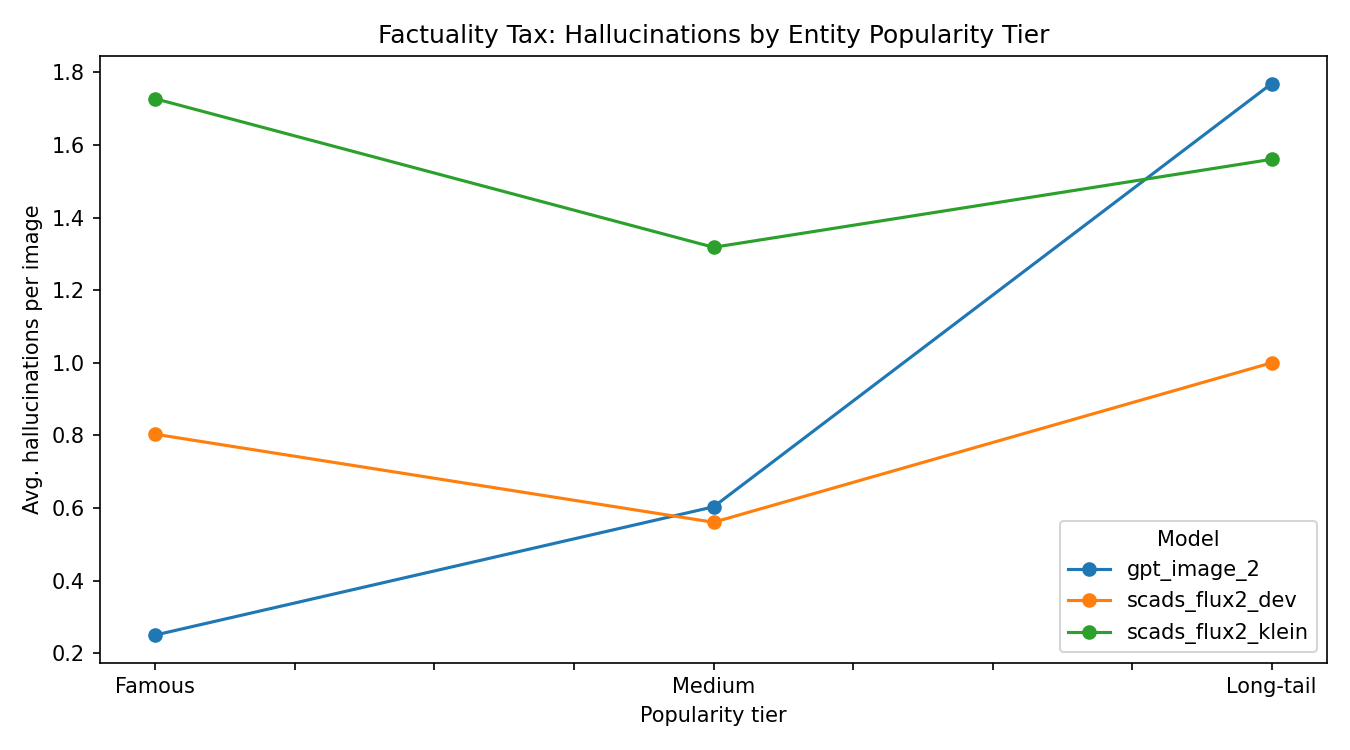
\includegraphics[width=0.82\textwidth]{../Code/analysing/analysis_output/rq3_hallucination_tax_by_tier.png}
\caption{Mean hallucinations per image across popularity tiers.}
\label{fig:hallu-tier}
\end{figure}

\begin{figure}[ht]
\centering
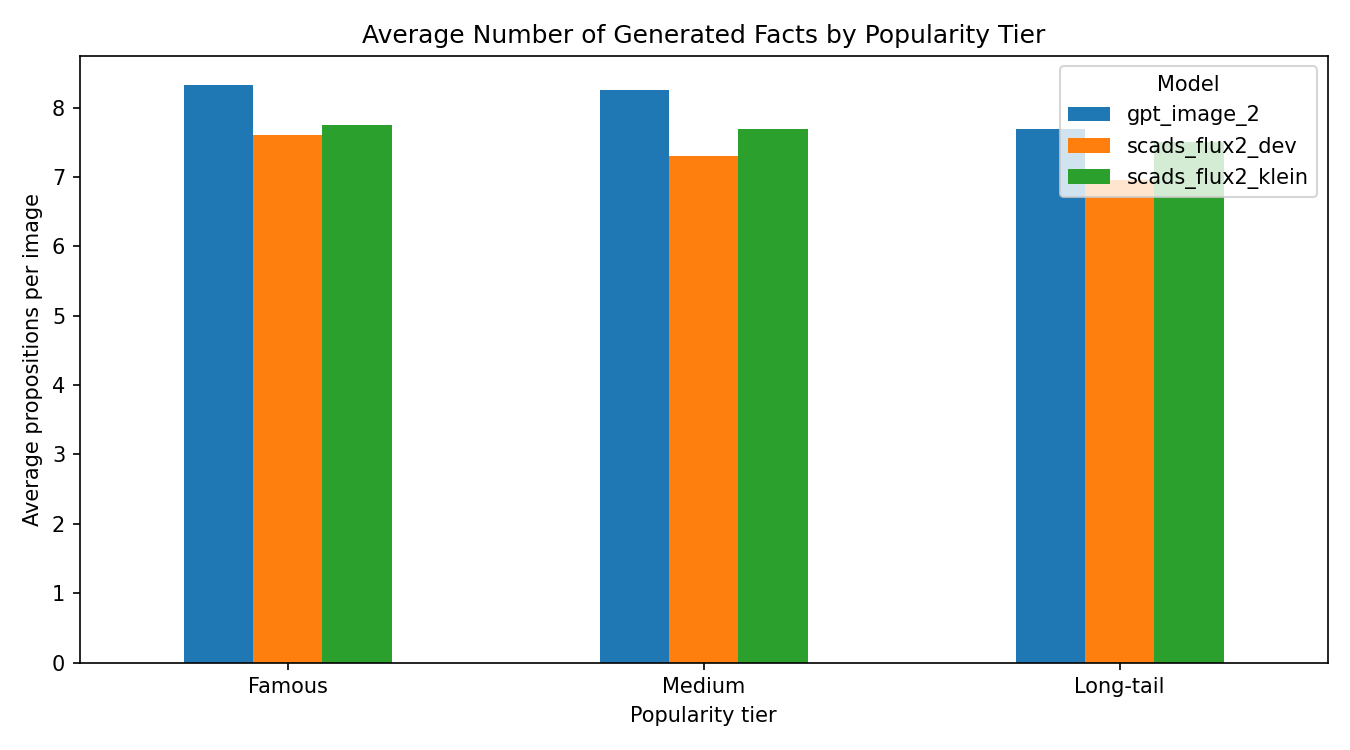
\includegraphics[width=0.82\textwidth]{../Code/analysing/analysis_output/rq3_average_facts_by_tier_fair.png}
\caption{Average number of generated propositions across popularity tiers.}
\label{fig:fact-tier}
\end{figure}

Figures~\ref{fig:hallu-tier} and~\ref{fig:fact-tier} should be read together.
The Long-tail tier does not consistently produce more propositions. In fact,
the average proposition count decreases for both FLUX models. The increase in
hallucination rate is therefore not explained by verbosity alone.

\section{Failure Cases and Refusals}

The missing-evaluation register contains nine GPT Image 2 entities refused by
the provider's safety system: Mahatma Gandhi, Frida Kahlo, Salvador Dali,
Transformers: Age of Extinction, Joker: Folie à Deux, Hugh Greenwood, Holby
City episode 1102, Treehouse of Horror, and Edouard Wojtczak. These refusals
cover both curated and Random entities. They are a property of the deployed
generation service and not an observation about the visual content of a
successful image.

This distinction is important for reproducibility. A benchmark that reports only
successful image rows would silently make the commercial model appear to have a
smaller test set. Conversely, assigning a zero score to a refusal would treat a
policy decision as factual ignorance. The present work reports coverage and
refusal counts separately and uses complete-case comparison for the main ranking.

\clearpage
\chapter{Discussion}

\section{Answers to the Research Questions}

For RQ1, all models frequently recover the coarse type of curated entities, but
none approaches perfect recognition. FLUX.2-dev performs best on type match.
For RQ2, the ranking changes: GPT Image 2 identifies distinctive features most
often, while FLUX.2-klein-4B is substantially weaker. This separation suggests
that entity recognition and entity-specific knowledge are different capabilities.

For RQ3, the models express propositions that are not supported by the reference
summaries. GPT Image 2 and FLUX.2-dev have similar overall rates. In contrast,
FLUX.2-klein-4B has nearly twice the rate of either model. Long-tail entities are
not simply harder because their images contain more claims; in several cases they
contain fewer claims but a higher fraction of unsupported claims.

\section{Implications and Limitations}

Visual plausibility is insufficient for using T2I outputs in knowledge-oriented
settings. A generated image may get the entity type right while failing to
include the feature that makes the entity recognizable. Conversely, an image can
look detailed while containing unsupported contextual elements. Proposition-level
checking is therefore a useful complement to image-quality metrics.

The safety refusals are a separate availability constraint, not a factual error.
The benchmark is also deliberately stratified and does not reproduce the natural
distribution of Wikipedia entities. The factual reference is a Wikipedia lead
summary, so a visible detail may be true while absent from the summary. The VLM
judge can make classification errors, and the curated subset is relatively small.
Finally, proposition count is only a proxy for visual information density: a
longer description is not necessarily more informative, and a shorter one is not
necessarily more accurate.

\chapter{Conclusion and Future Work}

This thesis introduced a benchmark for measuring factual knowledge in T2I models.
It evaluated type recognition, distinctive feature presence, and the truthfulness
of atomic visual propositions under a zero-context prompt. The experiments show
that T2I models contain non-trivial factual knowledge, but that this knowledge is
uneven across entity types and popularity tiers. Correct coarse type recognition
does not guarantee correct entity-specific features, and visually detailed images
can contain unsupported facts.

Future work should use multiple independent judges and human verification for a
sample of propositions. Reference information could be expanded beyond
Wikipedia leads to distinguish a false fact from a fact omitted by the summary.
The benchmark could also include repeated generations per entity, confidence
intervals, and additional models. A larger and naturally sampled Long-tail set
would allow stronger conclusions about factual knowledge across the distribution
of knowledge-base entities.

\appendix
\chapter{Supplementary Evaluation Information}

\section{Missing Entity--Model Pairs}

Table~\ref{tab:missing-eval} lists the missing evaluations identified from the
generation failure log. All rows belong to GPT Image 2 and all are safety
refusals. The complete CSV register, including provider error details, is stored
with the analysis outputs.

\begin{table}[ht]
\centering
\caption{Missing GPT Image 2 evaluations.}
\label{tab:missing-eval}
\begin{tabular}{lp{4.7cm}}
\toprule
Entity & Recorded reason \\
\midrule
Mahatma Gandhi & Safety refusal \\
Frida Kahlo & Safety refusal \\
Salvador Dali & Safety refusal \\
Transformers: Age of Extinction & Safety refusal \\
Joker: Folie à Deux & Safety refusal \\
Hugh Greenwood & Safety refusal \\
Holby City episode 1102 & Safety refusal \\
Treehouse of Horror & Safety refusal \\
Edouard Wojtczak & Safety refusal \\
\bottomrule
\end{tabular}
\end{table}

\section{Reproducibility Files}

The benchmark entities are stored in the entity CSV. Generated images are
organized by model and category. The evaluation results contain one row per
successful entity--model pair. The analysis script regenerates coverage tables,
fair comparisons, tier-level hallucination tables, proposition-count tables,
correlations, and figures from these inputs. This separation between raw rows
and derived tables allows the reported values to be recomputed after changing a
metric or adding another model.

\bibliographystyle{template/acl_natbib}
\bibliography{references}